\documentclass[11pt, a4paper]{memoir}
\usepackage[english, science, dropcaps, hyperref, submissionstatement]{ku-frontpage}
\usepackage[utf8]{inputenc}

\usepackage{pdfpages}
\usepackage{mathrsfs}
\usepackage{amsfonts}
\usepackage{amsmath}
\usepackage{mathtools}
\DeclareMathOperator\arctanh{arctanh}
\usepackage{amssymb}
\usepackage{bbm}
\usepackage{amsthm}
\usepackage{graphicx}
\usepackage{centernot}
\usepackage{caption}
\usepackage{subcaption}
\usepackage{braket}
\usepackage{lastpage}
\usepackage{enumitem}
\usepackage{setspace}
\usepackage{xcolor}
\usepackage[english]{babel} 
\usepackage{dsfont}


\usepackage[square,sort,comma,numbers]{natbib}
%\usepackage[colorlinks=true,allcolors=blue]{hyperref}

\usepackage{fancyhdr}

\newcommand{\euler}[1]{\text{e}^{#1}}
\newcommand{\Real}{\text{Re}}
\newcommand{\Imag}{\text{Im}}
\newcommand{\supp}{\text{supp}}
\newcommand{\norm}[1]{\left\lVert #1 \right\rVert}
\newcommand{\abs}[1]{\left\lvert #1 \right\rvert}
\newcommand{\floor}[1]{\left\lfloor #1 \right\rfloor}
\newcommand{\Span}[1]{\text{span}\left(#1\right)}
\newcommand{\dom}[1]{\mathcal D\left(#1\right)}
\newcommand{\Ran}[1]{\text{Ran}\left(#1\right)}
\newcommand{\conv}[1]{\text{co}\left\{#1\right\}}
\newcommand{\Ext}[1]{\text{Ext}\left\{#1\right\}}
\newcommand{\vertin}{\rotatebox[origin=c]{-90}{$\in$}}
\newcommand{\interior}[1]{%
	{\kern0pt#1}^{\mathrm{o}}%
}
\renewcommand{\braket}[1]{\left\langle#1\right\rangle}
\newcommand{\ketbra}[2]{\left\vert #1\middle\rangle\middle\langle #2 \right\vert}
\newcommand*\diff{\mathop{}\!\mathrm{d}}
\newcommand{\ie}{\emph{i.e.} }
\newcommand{\eg}{\emph{e.g.} }
\newcommand{\dd}{\partial }
\newcommand{\R}{\mathbb{R}}
\newcommand{\C}{\mathbb{C}}
\newcommand{\w}{\mathsf{w}}
\newcommand{\rr}{\mathcal{R}}


\newcommand{\Gliminf}{\Gamma\text{-}\liminf}
\newcommand{\Glimsup}{\Gamma\text{-}\limsup}
\newcommand{\Glim}{\Gamma\text{-}\lim}

\newtheorem{theorem}{Theorem}
\newtheorem{definition}[theorem]{Definition}
\newtheorem{proposition}[theorem]{Proposition}
\newtheorem{lemma}[theorem]{Lemma}
\newtheorem{corollary}[theorem]{Corollary}
\newtheorem{remark}[theorem]{Remark}

\numberwithin{equation}{section}

\linespread{1.3}

\setlength\arraycolsep{2 pt}
\setcounter{tocdepth}{2}
\setcounter{secnumdepth}{0}

\assignment{PhD thesis}
\author{Johannes Agerskov}

% The following are only needed if the \author, \title, \subtitle, and \date
% commands are not patchable. See the readme for more information.
\frontpageauthor{Johannes Agerskov}
\frontpagetitle{One Dimensional Dilute Quantum Gases and Their Ground State Energies}
%\frontpagesubtitle{An intruiging subtitle}
\frontpagedate{Submitted: March 30, 2023}

\title{One Dimensional Dilute Quantum Gases and Their Ground State Energies}
\subtitle{}
\date{Submitted: March 30, 2023}
\advisor{Advisor: Jan Philip Solovej}
%\frontpageimage{example.png}

\kupdfsetup{One Dimensional Dilute Quantum Gases and Their Ground State Energies}{}{Johannes Agerskov}

\begin{document}
\begingroup
  \fontencoding{T1}\fontfamily{LinuxLibertineT-OsF}\selectfont
  \maketitle
\endgroup

\tableofcontents

 \chapter{Introduction}
Since the seminal work of Lee, Huang, and Yang in 1957 \cite{lee1957eigenvalues, lee1957many, huang1957quantum}, there has been a tremendous interest in dilute quantum gases and their ground state energy expansions. Finding good approximations for the bosonic ground state energy, at least in two and three dimensions, is intimately related to understanding the formation of Bose-Einstein condensates. Furthermore, such ground state energy expansions often exhibit universality. More specifically, the ground state energy of dilute systems tends to depend on the interaction potential only through the scattering length. This interest has in the mathematical physics literature grown during the last decades culminating in the recent completion of a rigorous proof of the Lee-Huang-Yang formula in 2019 \cite{yau2009second,fournais2020energy}\footnote{While the lower bound was made fully general in terms of assumptions on the interaction potential in 2021 \cite{fournais2021energy}, weakening the assumptions under which the upper bound can be proven is still an active field of research. }. With the problem essentially solved for the three dimensional Bose gas, it is natural to seek similar ground state energy expansions in other dimensions or with different particle statistics. Recently, the two dimensional bosonic ground state energy expansion was proven to analogous precision in \cite{fournais2022ground}, and previously the fermionic ground state energy expansions have been studied in both two and three dimensions \cite{lieb2005ground}.

The general one dimensional dilute Bose gas, or quantum gas in general, has been surprisingly little studied both in the physics and mathematics literature. This may be partly due to the presence of solvable models in one dimension. In 1963 Lieb and Liniger showed that the one dimensional Bose gas with point (delta-function) interactions is solvable by Bethe ansatz \cite{lieb1963exact}. In practice, this means that one may obtain algebraic equations for the ground state and excited energies, by realizing the eigenstates to be superpositions of plane waves with suitable scattering boundary conditions. Similarly, in 1967, the one dimensional spin--$ 1/2 $ Fermi gas with point interactions was shown, in the physics literature, to be solvable by means of a generalized Bethe ansatz \cite{yang1967some}. This argument was one year later further generalized to accommodate any symmetry of the domain and hence any spin \cite{sutherland1968further}. Some effort has since then gone into arguing that various confined three dimensional systems may be well approximated by such point interacting systems in one dimension, leaving the analysis of the spectrum already complete \cite{olshanii1998atomic,petrov2000regimes,dunjko2001bosons,lieb2003one,lieb2004one,seiringer2008lieb}. In \cite{lieb2003one,lieb2004one,seiringer2008lieb} it was shown that such an approximation indeed is valid in certain confinement regimes. We call this regime the \emph{weak confinement regime}, and it is described by having the trapping length scale, in the transverse direction much longer than the three dimensional scattering length scale. This means that transverse excitations cannot be neglected. On the other hand, one may instead consider the \emph{strong confinement regime}, described by having the transverse trapping length scale much shorter than the scattering length scale. In this regime, the spectrum will presumably be well described by a purely one dimensional system, with the three dimensional potential simply restricted to a line. A crucial difference in this case, is that the one dimensional scattering length arising from such confinements may be positive, as opposed to the effective Lieb-Liniger model in which the one dimensional scattering length always is negative.\\
In this thesis, we analyze ground state energies of general one dimensional dilute gasses. This covers the strongly point interacting models but further extends the result to models with positive scattering lengths. The ground state energy expansion for one dimensional dilute bosons and spin polarized fermions was recently obtained in \cite{agerskov2022ground}, which appears, in an edited version, as Chapter \ref{ChapterTheGroundStateEnergyOfTheOneDimensionalDiluteBoseGas} of this thesis. The expansion obtained will exhibit similar universality as in the three and two dimensional cases. However, one major difference is apparent in the analysis and phenomenology of the one dimensional gas: There is no Bose-Einstein condensation. This fact may be traced back to the celebrated theorem of Hohenberg, Mermin, and Wagner \cite{hohenberg1967existence,mermin1966absence}, which excludes longe-range order for one dimensional interacting systems. Thus the formation of a condensate is broken by the interaction in one dimension. This famous result is in agreement with the results found in this thesis, where we explicitly verify that the ground state energy shows greater similarity to energies arising from Slater determinant states than to energies arising from a condensate.\\
The proof of a ground state energy expansion for the one dimensional dilute Bose gas and spin polarized Fermi gas leaves the question of whether there is a similar expansion for the total ground state of the spin--$ 1/2 $ fermionic system. Such an expansion is conjectured in Chapter \ref{ChapterTheGroundStateEnergyOfTheOneDimensionalDiluteBoseGas} (\cite{agerskov2022ground}), based on the solvable models at hand for such a system. We present in Chapter \ref{ChapterTheGroundStateEnergyOfTheOneDimensionalDiluteSpin1/2FermiGas} a proof of an upper bound matching this conjecture. In the proof, we define a trial state in which the spin part is determined variationally. Interestingly, the variational problem determining the spin part is that of the one dimensional Heisenberg chain. In the case of the usual spin--$ 1/2 $ fermions, we get the antiferromagnetic Heisenberg chain. However, we will show that for models of a different symmetry or with spin-dependent potentials, the spin chain may be both ferro- or antiferromagnetic. Furthermore, we will present an idea of how to prove a corresponding lower bound. We do this by proving results that are analogous to findings of Chapter \ref{ChapterTheGroundStateEnergyOfTheOneDimensionalDiluteBoseGas} (\cite{agerskov2022ground}). However, it will be apparent that certain results do not generalize for the spin--$ 1/2 $ Fermi system straightforwardly. We then present a conjecture which, if proven true, allows us to complete the generalization of the Chapter \ref{ChapterTheGroundStateEnergyOfTheOneDimensionalDiluteBoseGas} results. We give heuristic arguments for the validity of this conjecture, but also highlight where these arguments are lacking in mathematical rigor. Finally, we notice that the result of Chapter \ref{ChapterTheGroundStateEnergyOfTheOneDimensionalDiluteBoseGas} do generalize for spin--$ 1/2 $ systems with other symmetries or spin-dependent potentials exactly when the system is in a ferromagnetic phase.\\

We summarize here overall the structure of this thesis: In Chapter \ref{ChapterMany-BodyQuantumMechanics}, we review relevant concepts in many-body quantum mechanics. Furthermore, since we will allow for quite general interactions in the later analysis, we review under which conditions on the interaction potential the dynamics of quantum systems can be defined in terms of a lower bounded self-adjoint Hamiltonian. We prove a result stating that in one dimension this is possible for any interaction potential that is the sum of a $ \sigma $-finite measure and an absolutely continuous measure. After this we review the concept of diluteness and known results about dilute quantum gases. Finally, we both review and prove certain result about two solvable models in one dimension. In Chapter \ref{ChapterTheGroundStateEnergyOfTheOneDimensionalDiluteBoseGas}, we find and prove ground state energy expansions for both the one dimensional Bose and spin polarized Fermi gas. In Chapter \ref{ChapterTheGroundStateEnergyOfTheOneDimensionalDiluteSpin1/2FermiGas}, we generalize some results from Chapter \ref{ChapterTheGroundStateEnergyOfTheOneDimensionalDiluteBoseGas} in order to prove an upper bound on the ground state energy of the one dimensional dilute spin--$ 1/2 $ Fermi gas. Furthermore, we generalize certain results related to the lower bound in Chapter \ref{ChapterTheGroundStateEnergyOfTheOneDimensionalDiluteBoseGas}. Finally, we notice that completing the proof of a lower bound for the spin--$ 1/2 $ Fermi gas, is possible by proving a conjecture on the ground state energy of a model known as the Lieb-Liniger-Heisenberg model in its antiferromagnetic phase. We also note, in the ferromagnetic phase, that a tight lower bound on the Lieb-Liniger-Heisenberg model is trivially valid. Thus for certain other symmetries or spin-dependent potential, we find a tight lower bound exactly when they are in a ferromagnetic phase in this sense.
In Chapter \ref{ChapterConclusionAndOutlook}, we give a final summary of our findings and discuss open problems.


% !TeX spellcheck = en_US
\chapter{Many-Body Quantum Mechanics}
	In this chapter we give a brief introduction to many-body quantum mechanics. The chapter will serve to define relevant quantities, to set up the mathematical framework, and to state some preliminary results.

\section{Many-body Wave Functions}
	In quantum mechanics a system is described by a \emph{state} or \emph{wave function} in an underlying Hilbert space. 
	\begin{definition}
		A quantum system at fixed time is a pair \begin{equation*}
			(\Psi,\mathcal{H}),\text{ with } \Psi\in\mathcal{H} \text{ and } \norm{\Psi}=1,
		\end{equation*}
		where $ \mathcal{H} $ is a Hilbert space. Here $ \Psi $ is called the state or wave function of the system.
	\end{definition}
	In this thesis, we are mostly interested in quantum system consisting of $ N $ particles in a region $ \Omega\subseteq \R^d $, possibly with spin degrees of freedom $ \{S_i\}_{i\in{1,\ldots,N}} $. We refer to $ d $ as the \emph{dimension} of the system. Such a system is described by having $$ \mathcal{H}= L^2\left(\prod_{i=1}^{N}\left(\Omega\times \{-S_i,...,S_i\}\right) \right)=\otimes_{i=1}^{N}L^2\left(\Omega;\C^{2S_i+1}\right), $$ where $ S_i $ is the \emph{spin} of the $ i $th particle. Since we are more specifically interested in identical particles we will further restrict the structure of the underlying Hilbert space below.

	\subsection{Identical Particles: Bosons and Fermions}
		In the case when the particles in question are identical, \ie indistinguishable, it turn out that one can restrict the underlying Hilbert space, to have certain symmetries. Considering $ N $ indistinguishable particles, we restrict to the physical configuration space to $ C_{p,N}=C_N/S_N $, with $ C_N:=\{(x_1,\ldots,x_N)\in \Omega^N \vert x_i\neq x_j \text{ if }i\neq j\} $ on which the symmetric group act freely. For $ d\geq 2 $, we then require the wave function of the system to take values in a unitary irreducible representation of the fundamental group $\pi_1(C_{p,N})$, where we noted that the physical configuration space is path-connected in order for $ \pi_1(C_{p,N},x) $ to be independent of $ x\in C_{p,N} $.
		\begin{remark}
			For $ d\geq 3 $ we have $\pi_1(C_{p,N})=S_N$, for $ d=2 $ we have $\pi_1(C_{p,N})=B_N$ and for $d=1$ we have $\pi_1(C_{p,N})=\{1\}$. In the somewhat special case of $d=1$, $C_{p,N}=\{x_1<x_2<\ldots<x_N\}$. On this configuration space one can never interchange particles without crossing the singular excluded incidence (hyper)planes. Thus the allowed particle statistics are determined by the possible permutation invariant dynamics (see section below) on this space. In section ... we will see examples of different particle statistics in one dimension. 
		\end{remark}
		\begin{remark}
			Adding spin to the above considerations amounts to having $C_N:=\{(z_1,\ldots,z_N)\in \left(\Omega\times\{-S,\ldots,S\}\right)^N \vert (z_i)_1\neq (z_j)_1 \text{ if }i\neq j\}$, and $C_{p,N}:=C_N/S_N$. In this case $C_{p,N}$ is not path connected, however, for each configuration of spins $ \sigma=(\sigma_1,\ldots,\sigma_N)\in\{-S,\ldots,S\}^N $ the configurations spaces $ C_{p,N,\sigma}=\{((x_1,\sigma_1),\ldots,(x_N,\sigma_N))\in \left(\Omega\times\{-S,\ldots,S\}\right)^N \vert x_i\neq x_j \text{ if }i\neq j\} $ are path connected and their fundamental groups are isomorphic to the fundamental group in the spinless case independent of $ \sigma $.\\
			Alternatively, one can view the wave function as a $ (2S+1)^N $-dimensional vector bundle over the physical (spinless) configuration space.
		\end{remark}
		In the remaining part of this thesis, we will mainly be interested in the two irreducible representations that are the symmetric representation and the anti-symmetric representation, in which we refer to the particles as \emph{bosons} and \emph{fermions} respectively. It is an empirical fact that bosons and fermions are the only types of elementary particles that are encountered in nature. Hence for bosons we restrict to wave functions in the symmetric (or bosonic) subspace $ L^2_{s}\left(\left(\Omega\times \{-S,\ldots,S\}\right)^N \right)\cong\vee_{i=1}^{N}L^2\left(\Omega; \C^{2S+1}\right)$ and for fermions we restrict to wave-functions in the anti-symmetric (or fermionic) subspace $ L^2_{a}\left(\left(\Omega\times \{-S,\ldots,S\}\right)^N \right)\cong\wedge_{i=1}^{N}L^2\left(\Omega; \C^{2S+1}\right)$.\\
		To recap we list the following important definitions
		\begin{definition}
			A quantum system of $N$ spin--$ S $ bosons in $ \Omega\subseteq\R^d $ at fixed time is a pair
			\begin{equation*}
			(\Psi,\mathcal{H}),\text{ with } \Psi\in\mathcal{H}\text{ and }\norm{\Psi}=1,
			\end{equation*}
			where $ \mathcal{H}=L^2_{s}\left(\left(\Omega\times \{-S,\ldots,S\}\right)^N \right)\cong\vee_{i=1}^{N}L^2\left(\Omega; \C^{2S+1}\right) $.
		\end{definition}
		\begin{definition}
			A quantum system of $N$ spin--$ S $ fermions in $ \Omega\subseteq\R^d $ at fixed time is a pair
			\begin{equation*}
			(\Psi,\mathcal{H}),\text{ with } \Psi\in\mathcal{H}\text{ and }\norm{\Psi}=1,
			\end{equation*}
			where $ \mathcal{H}=L^2_{a}\left(\left(\Omega\times \{-S,\ldots,S\}\right)^N \right)\cong\wedge_{i=1}^{N}L^2\left(\Omega; \C^{2S+1}\right) $.
		\end{definition}
	
\section{Observables, Dynamics, and Energy}
In general we call any self-adjoint operator on $ \mathcal{H} $ an \emph{observable}. Physically, observables represent quantities that, in principle, can be measured in an experiment. It is a postulate of quantum mechanics that given an observable $ \mathcal{O}=\int_{\sigma(\mathcal{O})}\lambda \diff P_\lambda $, where $\{P_\lambda\}_{\lambda\in\sigma(\mathcal{O})}$ is the projection valued measure associated to $ \mathcal{O} $ by the spectral theorem \cite{reed1981functional}, the probability of a measurement of $ \mathcal{O} $ in state $ \Psi\in\dom{\mathcal{O}} $ having outcome $ \lambda\in M\subset \R $ is given by $ P\left((\mathcal{O},\Psi)\rightarrow\lambda\in M\right)=\int_{\lambda\in M} \braket{\Psi,P_\lambda\Psi} $. 
Furhtermore we defined the expected value of an observable.
\begin{definition}
	The \textbf{expectation value} of an observable $ \mathcal{O} $ in state $ \Psi\in\dom{\mathcal{O}} $ is 
	$$ \braket{\mathcal{O}}_\Psi:=\int_{\lambda\in\sigma(\mathcal{O})}\lambda\braket{\Psi,P_\lambda\Psi} $$
	where $\{P_\lambda\}_{\lambda\in\sigma(\mathcal{O})}$ is the projection valued measure associated to $ \mathcal{O} $ by the spectral theorem.
\end{definition}


I the previous section we defined a quantum system at a fixed time. However, we are often interested in dynamics of the system. In quantum mechanics, time evolution is modeled by the infinitesimal generator of time evolution, $ H $, also known as the \emph{Hamiltonian}. We will in this thesis take $ H $ to be a (time-independent) lower bounded self-adjoint operator on $ \mathcal{H} $. A state evolves in time according to the Schr\"odinger equation\begin{equation*}
\Psi(t)=\exp\left(-iH(t-t_0)\right)\Psi(t_0),
\end{equation*}
where have set $ \hbar=1 $.
\begin{remark}
	By Stone's theorem (ref Reed and Simon), the existance of a self-adjoint Hamiltonian, $ H $, is guaranteed for any time evolution described by $ \Psi(t)=U(t-t_0)\Psi(t_0) $, when $ U(t) $ is a strongly continuous one-parameter unitary group.
\end{remark}
Since the Hamiltonian, $ H $, is self-adjoint, it represents an observable which we call \emph{energy}. Since $ H $ is lower bounded, there is a natural notion of lowest energy of $ H $.
\begin{definition}
	The \textbf{ground state energy} of $ H $ is defined by 
	$$
	E_0(H):=\inf(\sigma(H))
	$$
\end{definition}
Furthermore, we define the notion of a \emph{ground state} of $ H $ as
\begin{definition}
	We say that a (normalized) state $ \Psi\in \dom{H}\subset \mathcal{H} $ is a \textbf{ground state} of $ H $ if $$ \braket{H}_\Psi=E_0(H). $$
\end{definition}
When studying ground states and ground state energies it is useful to have the following variational characterization.
\begin{remark}\label{RemarkVariationalPrinciple1}
	It follows from the spectral theorem (ref Reed and Simon) that the ground state energy is given by \begin{equation}\label{EqVariationalGroundStateEnergyOperator}
		E_0(H)=\inf_{\Psi\in \dom{\mathcal{H}}}\frac{\braket{\Psi,H\Psi}}{\norm{\Psi}^2}.
	\end{equation}
\end{remark}
\begin{remark}
	It is straightforward to show that the quadratic form $ \dom{H}\ni\Psi\mapsto\braket{\Psi,H\Psi} $ is lower bounded and closable, since $ H $ is lower bounded and self-adjoint.
\end{remark}
\begin{definition}
	Given a Hamiltonian, $ H $, we define the \textbf{associated energy quadratic form}, $ \mathcal{E}_H:\mathcal{\dom{\mathcal{E}_H}}\to \R $, as the closure of the quadratic form $ \dom{H}\ni\Psi\mapsto\braket{\Psi,H\Psi} $. When $ H $ is given from the context, we will often write $ \mathcal{E} $ as short for $ \mathcal{E}_H $.
\end{definition}
\begin{remark}\label{RemarkVariationalPrinciple2}
	From the definition of $\mathcal{E_H}$ and from Remark \ref{RemarkVariationalPrinciple1} it follows straightforwardly that we have \begin{equation}\label{EqVariationalGroundStateEnergyForm}
		E_0(H)=\inf_{\Psi\in \dom{\mathcal{E_H}}}\frac{\mathcal{E_H}(\Psi)}{\abs{\Psi}^2}=\inf_{\substack{\Psi\in \dom{\mathcal{E_H}},\\\norm{\Psi}=1}}\mathcal{E_H}(\Psi), 
	\end{equation}
	as $ \dom{H} $ is form core for $\mathcal{E_H}$.
\end{remark}
We refer to both \eqref{EqVariationalGroundStateEnergyOperator} and \eqref{EqVariationalGroundStateEnergyForm} as \emph{the variational principle}.
We will often in the remaining take \eqref{EqVariationalGroundStateEnergyForm} as the vary definition of the ground state energy. Furthermore, one can also define the dynamics of a quantum system by specifying an energy quadratic form in the following sense
\begin{remark}[Ref!!]\label{RemarkOperatorFromQuadraticForm}
	Given a densely defined, lower bounded, closable, quadratic form $ \mathcal{E}:\dom{\mathcal{E}}\to \R $ there exist a \textbf{unique} lower bounded, self-adjoint operator $ H_\mathcal{E} $, such that $ \mathcal{E}(\Psi)=\braket{\Psi,H_\mathcal{E}\Psi} $ for all $ \Psi\in \dom{H_\mathcal{E}} $, and $ \dom{H_\mathcal{E}} $ is form core for $\overline{\mathcal{E}}$, \ie the form closure of $ \braket{\cdot,H_\mathcal{E}\cdot} $ is equal to the form closure of $\mathcal{E}$. 
\end{remark}
Thus we will frequently change between the two equivalent formulations of the dynamics of a quantum system that are the operator, $ H $, formulation and the quadratic form, $ \mathcal{E} $, formulation
\subsection{Many-Body Hamiltonians}
Until this point, we have not specified the class of Hamiltonians that we will be interested in. We have seen, that we will care mainly about Hamiltonians defined on the bosonic or fermionic subspace, however no specification has been made about the dynamics on these subspaces. We are interested in modeling $ N $ particles in some region $ \Omega\subseteq\R^d $ that interact locally with each other. For the remaining of this subsection we will ignore spin, knowing that including spin degrees of freedom is completely analogous. In practice, and for suitably mild interactions, this means that the Hamiltonian \emph{formally} (meaning restricted to the fermionic or bosonic subspace of $ C^\infty_0(\Omega^N) $) takes the form \begin{equation}
H=\sum_{i=1}^{N}T_i+U(x_1,\ldots,x_N)
\end{equation}
where $ T_i $ is the \emph{kinetic energy operator} for particle $ i $ and the \emph{potential} $ U $ is a multiplication operator which models the local interaction among the particles. The kinetic energy operator is taken to be\footnote{This is usually justified by going through a canonical quantization procedure for the classical Hamiltonian function of the system we are interested in modeling} \begin{equation}
T_i=-\frac{1}{2m_i}\Delta_i\qquad (\hbar=1)
\end{equation} 
since we interested in identical particles, we will from this point onward choose $ m_i=1/2 $. As for the potential, $ V $, we of course immediately restrict to permutation-invariant function, $ U $, for identical particles. However, in the following we will further restrict to a combination of having a trapping potential and radial pair potentials, which model pairwise interactions that only depend on the distances between particles. Such potentials take the form \begin{equation}
U(x_1,\ldots,x_N)=\sum_{i<j} v(x_i-x_j) + \sum_{i=1}^{N}V(x_i)
\end{equation}
where we take $ v $ to be a radial function and, $ V $, is called the \emph{trapping potential}. We will generally take $ v $ to be repulsive, meaning $ v\geq 0 $, with compact support. The trapping potential we will disregard \ie $ V=0 $. We will then in general take the true Hamiltonian to be a self-adjoint extensions of the symmetric \emph{formal} Hamiltonian. Now some models of stronger interactions, \eg the hard core interaction, requires a more delicate construction with respect to the initial definition of the formal Hamiltonian. However, the construction of the Hamiltonian can be done in a more unified manner when constructing the energy quadratic form. 
\begin{definition}
	For a system of $ N $ bosons/fermions in region $ \Omega\in\R^d $, we define for $ \sigma\in[0,\infty] $ \textbf{the energy quadratic forms}
\begin{equation}\label{key}
\mathcal{E}_{(v,\sigma)}(\Psi)=\int_{\Omega^N} \sum_{i=1}^{N}\abs{\nabla_i\Psi}^2+\sum_{i<j} v(x_i-x_j)\abs{\Psi}^2+\sigma\int_{\dd (\Omega^N)}\abs{\Psi}^2,
\end{equation}
with domain $ \dom{\mathcal{E}_{(v,\sigma)}}=\{\Psi\in (C^\infty_0(\Omega^N))_{\text{b/f}}\vert \mathcal{E}_{(v,\sigma)}(\Psi)<\infty\} $. with $ (C^\infty_0(\Omega^N))_{\text{b/f}} $ meaning the bosonic/fermionic subspace of $ C^\infty_0(\Omega^N) $. $ \sigma=\infty $ is taken to mean Dirichlet boundary conditions.
\end{definition}
Of course $ \mathcal{E}_{(v,\sigma)}\geq 0 $ for any $ \sigma\in[0,\infty] $ and $ v\geq 0 $. However, the closability of $ \mathcal{E}_{(v,\sigma)} $ is not evident. In fact for general $ v $, $ \mathcal{E}_{(v,\sigma)} $ will not be neither densely defined nor closable on $ L^2_{s/a}(\Omega^N) $. However, it will both densely defined on a closed subspace $ \mathcal{H}_{(v,\sigma)}:=\overline{\dom{\mathcal{E}_{(v,\sigma)}}}^{\norm{\cdot}_2} $ of $ L^2_{s/a}(\Omega^N) $, hence we take $ \mathcal{H}_{(v,\sigma)} $ to be the Hilbert space of the system, when this is the case. Closability of $ \mathcal{E}_{(v,\sigma)} $ on $ \mathcal{H}_{(v,\sigma)} $ is not necessarily satisfied. Thus we make the following definition
\begin{definition}
	We say a potential $ v\geq 0 $ is \textbf{allowed} in dimension $ d $, if $ \mathcal{E}_{(v,\sigma)} $ is closable on $ \mathcal{H}_{(v,\sigma)}:=\overline{\dom{\mathcal{E}_{(v,\sigma)}}}^{\norm{\cdot}_2}\subset L^2_{s/a}(\Omega^N)$ for any $ \sigma\in[0,\infty] $.
\end{definition}
\begin{remark}
	There are plenty of allowed potentials, but the notion does depend on the dimension, $ d $. For example is $ v=\delta_0 $, \ie the delta function potential, allowed in dimension $ d=1 $, but not in dimension $ d\geq 2 $. This can be seen from the fact that for $ d=1 $ the incidence planes are co-dimension $ 1 $, and hence the trace theorem gives closability, but for $ d\geq 2 $ where the incidence planes are of co-dimension $ \geq 2 $ it is known that the trace of $ H^1 $ is not contained in $ L^2 $. (Ref!!)
\end{remark}


\begin{remark} \label{RemarkdDimPotentialAllowed}
	For any radial $ v\geq 0 $ that is measurable  $\mathcal{E}_{(v,\sigma)} $ is the quadratic form associated to a self-adjoint operator on some Hilbert space $ \mathcal{H}_{(v,\sigma)}\subset L^2_{s/a}(\Omega^N) $. It is well known that $\mathcal{E}_{(0,\sigma)}$ is closable on $ \mathcal{H}_{(0,\sigma)}\supseteq \mathcal{H}_{(v,\sigma)}    $, hence on $  \mathcal{H}_{(v,\sigma)} $. Thus closability of $ \mathcal{E}_{(v,\sigma)} $ amount to showing that $ \psi_n \xrightarrow{\norm{\cdot}_2}0 $ as $ n\to\infty $ and $ (\psi_n)_{n\in\mathbb{N}}\subset L^2\left(\Omega^N,\underbrace{\sum_{i<j}v(x_i-x_j)\diff\lambda^{N}}_{\coloneqq \diff\mu_v}\right) $ Cauchy, implies $ \psi_n\xrightarrow{\norm{\cdot}_{L^2(\Omega^N,\diff\mu_v)}}0  $. This is evident from the fact that $\psi_n\xrightarrow{\norm{\cdot}_{L^2(\Omega^N,\diff\mu_v)}}f$ for some $ f\in L^2(\Omega^N,\diff\mu_v) $ by completeness. Now $ \psi_n $ has a subsequence that converges $ \lambda^{N} $--almost everywhere to $ 0 $, and this subsequence further has a subsequence that converges $ \mu_v $--almost everywhere to $ f $. Hence $ f=0 $ $ \mu_v $--almost everywhere, as $ \mu_v\ll \lambda^N $. \\
	Thus there is a corresponding self-adjoint operator $ H_{(v,\sigma)} $ to $ \mathcal{E}_{(v,\sigma)} $ on $ \mathcal{H}_{(v,\sigma)} $, which we shall formally write as $ H_{(v,\sigma)}=-\sum_{i=1}^{N}\Delta_i+\sum_{1\leq i<j\leq N}v(x_i-x_j) $.
\end{remark}
The argument from the previous may be generalized slightly in the case of $ d=1 $, in order to show that any $ \sigma $--finite measure $ v\diff\lambda^{N} $ is allowed as potential. Notice that we slightly abuse notation and write $ v(x_i-x_j)\diff\lambda^N $ even when $ v $ is a singular continuous measure and thus has no density. However, we do think of $ v $ a being a one-dimensional measure in the sense that 
$$ v(x_i-x_j)\diff\lambda^N:=\diff\mu_{v_{ij}}\times \diff \lambda^{N-1}_{(x_i-x_j)=\text{ fixed}},  $$ 
where we defined $ \diff \mu_{v_{ij}}:=v(x_i-x_j)\diff (x_i-x_j) $ and $ \lambda^{N-1}_{(x_i-x_j)=\text{ fixed}} $ to be the measure such that $ \diff\lambda^{N}=\diff(x_i-x_j)\times \diff\lambda^{N-1}_{(x_i-x_j)=\text{ fixed}} $. Uniqueness of the product measure is guaranteed by $ \sigma $-finiteness of $ v $.
%\begin{lemma}
%	Let $ (f_n)_{n\in\mathbb{N}}\subset H^1(\Omega) $ be a sequence such that $ \norm{f_n}_{H^1}\to0 $ as $ n\to\infty $. Then $ f_n $ has a subsequence that converges pointwise to 0 on $ \lambda^{N-1} $--almost all lines.
%\end{lemma}
%\begin{proof}
%	We pass to a subsequence, which we also denote $ f_n$, such that $ f_n $ converges pointwise $ \lambda^N $--a.e. to $ 0 $. 
%	Since $ f_n\in H^1(\Omega) $, we know that $ f_n $ are absolutely continuous on $ \lambda^{N-1} $--almost all lines. Now consider the $ H^1(\R) $ norms of $ f_n $ along each line. Clearly these constitute $ L^2 $ functions, with norms converging to $ 0 $. Hence there exist a subsequence that converges pointwise $ \lambda^{N-1} $--almost everywhere to $ 0 $. Thus there is a subsequence such that for almost all lines, the $ H^1 $ norm along the line converges to zero. But then $ f_n $ converges, by Morrey's inequality, uniformly to 0 on almost all lines.
%\end{proof}
%precise statement. 
We will need the following essential lemma, where we use the notation  $ \lambda_k^{N-1}\coloneqq \prod_{i\neq k}\diff x_i $ 
\begin{lemma}\label{LemmaH1PointwiseConvergence}
	Let $ (f_n)_{n\in\mathbb{N}}\subset H^1(\Omega^N) $ be a sequence such that $ \norm{f_n}_{H^1}\to0 $ as $ n\to\infty $. Then defining $ f^k_n(t,\overline{x}^k)\coloneqq f_n(x_1,\ldots,x_{k-1},t,x_{k+1},\ldots,x_N) $ for any $ k=1,\ldots,N $, we have that $ (f^k_n)_{n\in\mathbb{N}} $ has a subsequence that converges pointwise (in $ t $) to $ 0 $, $ \lambda_k^{N-1} $--a.e. for all $ k=1,\ldots,N $.
\end{lemma}
\begin{proof}
	We pass first to a subsequence, which we also denote $ f_n$, such that $ f_n $ converges pointwise $ \lambda^N $--a.e. to $ 0 $. 
	Since $ f_n\in H^1(\Omega^N) $, we know for any $ k=1,\ldots,N $ that $ f^k_n(t,\overline{x}^k) $ are in $ H^1(\Omega) $ (as functions of t) $ \lambda_k^{N-1} $--a.e.
	[\cite{evans1991measure} Theorem 2 p. 164].
	Now consider the $ H^1(\Omega) $ norms of $ g_n^k(\overline{x}^k)\coloneqq \norm{f^k_n(\cdot,\overline{x}^k)}_{H^1(\Omega)} $. Clearly $ g_n^k $ constitute $ L^2 $ functions, with norms converging to $ 0 $. Hence there exist a subsequence that converges pointwise $ \lambda_k^{N-1} $--almost everywhere to $ 0 $. Then there is a subsequence $ f_{n_i}^k $ such that for $ \lambda_k^{N-1} $--a.e. $ \overline{x}^k $, $ f_{n_i}^k(\cdot,\overline{x}^k) $ converges to $ 0 $ in $ H^1(\Omega) $. But then $  f_{n_i}^k(\cdot,\overline{x}^k) $ converges, by Morrey's inequality, pointwise to $ 0 $.
\end{proof}
Using this lemma, we may prove the following Proposition
\begin{proposition}\label{Lemma1dPotentialAllowed}
	Let $ d=1 $, then for any $ \sigma $-finite measure, $ v $, we have that $ \mathcal{E}_{(v,\sigma)} $ is the quadratic form associated to a self adjoint operator $ H_{(v,\sigma)} $ on some Hilbert space $ \mathcal{H}_{(v,\sigma)} $.
\end{proposition}
\begin{proof}
	As previously, we define $\mathcal{H}_{(v,\sigma)}:=\overline{\dom{\mathcal{E}_{(v,\sigma)}}}^{\norm{\cdot}_2} $ and $ \diff\mu_v=\sum_{1\leq i<j\leq N}v(x_i-x_j)\diff\lambda^N $. Clearly $ \mathcal{E}_{(v,\sigma)} $ is lower bounded and densely defined in $ \mathcal{H}_{(v,\sigma)} $. Closability amounts to showing that $ \psi_n\xrightarrow{\norm{\cdot}_{L^2(\Omega^N,\diff\lambda^{N})}}0 $ and $ (\psi_n)_{n\in\mathbb{N}}\subset L^2\left(\Omega^N,\diff\mu_v\right) $ Cauchy w.r.t the norm $ \norm{\cdot}_{\mathcal{E}_{(v,\sigma)}}=\sqrt{\mathcal{E}_{(v,\sigma)}(\cdot)+\norm{\cdot}_2^2} $, implies $ \psi_n\xrightarrow{\norm{\cdot}_{L^2(\Omega^N,\diff\mu_v)}}0  $. Now since $ (\psi_n)_{n\in\mathbb{N}}$ is a Cauchy sequence in $ L^2\left(\Omega^N,\diff\mu_v\right) $, it has a subsequence that converges $ \mu_v $--almost everywhere to some function $ f\in L^2\left(\Omega^N,\diff\mu_v\right)  $. Furthermore, this subsequence has a further subsequence that converges $ \lambda^{N} $--almost everywhere to $ 0 $. However, since $ (\psi_n)_{n\in\mathbb{N}}$ converges to $ 0 $ in $ H^1(\Omega^N,\diff \lambda^N) $, Lemma \ref{LemmaH1PointwiseConvergence} implies that for $ (x_i-x_j) $ fixed $ (\psi_n)_{n\in\mathbb{N}} $ converges $ \lambda^{N-1} $--a.e. to $ 0 $. Hence $ \left(\psi_n\right)_{n\in\mathbb{N}} $ converges pointwise to $ 0 $ on $ \lambda^{N-1} $--almost all lines. Now notice that $ \diff \mu_v=\sum_{1\leq i<j\leq N} \diff \mu_{v_{ij}}\times \diff\lambda^{N-1}_{(x_i-x_j)=\text{ fixed}} $. Thus for $ \lambda^{N-1}_{(x_i-x_j)=\text{ fixed}} $--almost all lines in $ \Omega^N $ with $ x_i+x_j $ and $ x_k $ fixed for all $ k\neq i,j $, by passing to a subsequence $ \psi_n $ converges pointwise to $ 0 $, by Lemma \ref{LemmaH1PointwiseConvergence}. But also on $ \lambda^{N-1}_{(x_i-x_j)=\text{ fixed}} $--almost all these lines $ \psi_n $ converges $ \mu_{v_{ij}} $--almost everywhere to $ f $, and hence $ f=0 $ $ \mu_{v_{ij}} $--almost everywhere. Thus we conclude that $ f=0 $ $ \mu_v $--almost everywhere. The lemma now follows from Remark \ref{RemarkOperatorFromQuadraticForm}.
\end{proof}
\begin{remark}
	Combining Lemma \ref{Lemma1dPotentialAllowed} and Remark \ref{RemarkdDimPotentialAllowed} we conclude that potentials of the form $ v=v_{\sigma\text{--finite}}+v_{\text{abs.cont.}} $, where $ v_{\sigma\text{--finite}} $ is a $ \sigma $--finite measure and $ v_{\text{abs.cont.}} $ is an absolutely continuous measure (w.r.t. Lebesgue measure) are allowed in one dimension, $ d=1 $. We will in Chapter.... obtain result about the ground state energy of such systems.
\end{remark}
\begin{remark}
	We emphasize that one can construct dynamics of a quantum system that are not given by a pair potential in the sense of the discussion above. It is, for example, possible to study point interactions in $ d\geq 2 $, however, they cannot be seen as arising from a potential (\eg a $ \delta $-function potential). Instead, one studies in this case the self-adjoint extensions of the Laplacian on functions supported away from the incidence planes of the particles. \cite{albeverio2012solvable}.
\end{remark}


\section{The Scattering Length}
When analyzing dynamics of a quantum system, it is natural to define certain length scales, on which different processes take place. These length scales often play important roles in understanding the physics of the system, and thus often appear naturally in expressions for the energies of the system. One such length scale that will be of particular importance throughout this thesis is the \emph{scattering length}. The intuition behind the name is that scattering occurs on this length scale. This intuition will be of important throughout the thesis, and especially when  constructing low energy trial states in order to estimate ground state energies by applying the variational principle. The scattering length has multiple equivalent definitions in the literature, but we shall here define it conveniently from a variational principle.\\
Consider the two-body problem in $ \Omega=\R^d $ with a spherically symmetric positive potential of compact support $ v\geq 0 $. We allow for the potential, $ v $, to be a measure, when makes sense, \ie when it is \emph{allowed}. Let $ R_0>0 $ be such that $ \supp(v)\subset B_{R_0} $. Many assumptions on $ v $ can be weakened, but these conditions are sufficient for the scope of this thesis. The formal Hamiltonian can be written \begin{equation}
H_2=-\frac{1}{2m_1}\Delta_1-\frac{1}{2m_2}\Delta_2+v(x_1-x_2),
\end{equation}
For now we keep the masses, but we will be mostly interested in the case $ m_1=m_2=1/2 $. Defining the center of mass coordinate $ X=(m_1x_1+m_2x_2)/(m_1+m_2) $ and the relative coordinate $ y=x_1-x_2 $, we see that the kinetic energy may be rewritten \begin{equation}
\begin{aligned}
-\frac{1}{2m_1}\Delta_1-\frac{1}{2m_2}\Delta_2&=-\sum_{i=1}^{d}\frac{1}{2m_1}\left(\frac{\partial y_i}{\partial (x_1)_i}\partial_{y_i}+\frac{\partial X_i}{\partial (x_1)_i}\partial_{X_i}\right)^2\\&\qquad\qquad+\frac{1}{2m_2}\left(\frac{\partial y_i}{\partial (x_2)_i}\partial_{y_i}+\frac{\partial X_i}{\partial (x_2)_i}\partial_{X_i}\right)^2\\
&=-\sum_{i=1}^{d}\frac{1}{2m_1}\left(\partial_{y_i}+\frac{m_1}{m_1+m_2}\partial_{X_i}\right)^2\\&\qquad\qquad+\frac{1}{2m_2}\left(-\partial_{y_i}+\frac{m_2}{m_1+m_2}\partial_{X_i}\right)^2\\
&=-\frac{1}{2\mu}\Delta_y-\frac{1}{2(m_1+m_2)}\Delta_X,
\end{aligned}
\end{equation}
where $ \mu\coloneqq \frac{m_1m_2}{m_1+m_2} $. Thus we have separated the center of mass motion and the Hamiltonian may be decomposed \begin{equation}
H=H_{\text{CM}}+H_{\text{rel}},
\end{equation}
with $ H_{\text{CM}}=-\frac{1}{2(m_1+m_2)}\Delta_X $ and $ H_{\text{rel}}=-\frac{1}{2\mu}\Delta_y+v(y) $. In scattering theory, we will generally be interested in the relative motion of particles. A natural question is whether we can locally minimize the relative energy of the two particles when they are nearby? The answer is affirmative, which can be seen by the following:\\
Consider the ($ R $-local, relative) energy functional \begin{equation}
\mathcal{E}_R(\psi)=\int_{B_R} \frac{1}{2\mu}\abs{\nabla\psi}^2+v\abs{\psi}^2,
\end{equation}
with $ R>R_0 $. Then we have 
\begin{theorem}[Theorem A.1 in \cite{lieb2001ground}]\label{TheoremScatteringLength}
	Let $ R>R_0 $ then in the class of functions 
	$$ \{\phi\in H^1(B_R)\ \vert\ \phi(x)=1,\text{ for }x\in S_R\}, $$ with $ S_R $ the sphere of radius $ R $,
	there is a unique $ \phi_0 $ that minimizes $ \mathcal{E}_R $. This function is non-negative and spherically symmetric, $ \phi_0(x)=f_0(\abs{x}) $ for some $ f\geq 0 $, and it satisfies the equation\begin{equation}
	-\frac{1}{2\mu}\Delta\phi_0+v\phi_0=0,
	\end{equation}
	in the sense of distributions on $ B_R $.
	
	For $ R_0<r<R $ we have \begin{equation}
	f_0(r)=\begin{cases}
	(r-a)/(R-a)&\text{ for }d=1\\
	\ln(r/a)/\ln(R/a)& \text{ for }d=2\\
	(1-ar^{2-n})/(1-aR^{2-n})& \text{ for }d=3
	\end{cases}
	\end{equation}
	for some length, $ a $, which we call \textbf{the (s-wave) scattering length}.
	
	The minimum value of $ \mathcal{E}_R $ is 
	\begin{equation}
	f_0(r)=\begin{cases}
	1/\mu(R-a)&\text{ for }d=1\\
	\pi/[\mu\ln(R/a)]& \text{ for }d=2\\
	\pi^{n/2}a/[\mu\Gamma(n/2)(1-aR^{2-n})]& \text{ for }d=3.
	\end{cases}
	\end{equation}
\end{theorem}
We note that in $ d>3 $, the scattering length is not actually a length in the sense of units. This is purely an artifact of the conventions used in the definition.\\
The definition above defined only the s-wave scattering length. One can proceed to define different kinds of scattering lengths depending on which asymptotic behavior (boundary condition) we demand of the minimizer of $ \mathcal{E}_R $. We will be mostly interested in a different kind of scattering length in dimension $ d=1 $. Thus we define
\begin{definition}\label{DefinitionEvenScatteringLength}
	Let $ f_e\in H^1(\R) $ be the unique solutions of the equation\begin{equation}\label{EqEvenScatteringEquation}
	-f_e''(x)+v(x)f_e=0,
	\end{equation}
	in the sense of distributions on $ B_R $, with boundary conditions $ f_e(R)=1 $ and $ f_e(-R)=1 $. Then we have \begin{equation}
	\int_{B_R} 2\abs{f_e'}^2+v \abs{f_e}^2=\frac{4}{R-a_e},
	\end{equation} 
	for some length, $ a_e $, called the \textbf{even wave scattering length}.
\end{definition}
\begin{definition}\label{DefinitionOddScatteringLenght}
	Let $ f_o\in H^1(\R) $ be the unique solutions of the equation\begin{equation}\label{EqOddScatteringEquation}
	-f_o''(x)+v(x)f_o=0,
	\end{equation}
	in the sense of distributions on $ B_R $, with boundary conditions $ f_o(R)=1 $ and $ f_o(-R)=-1 $. Then we have \begin{equation}
	\int_{B_R} 2\abs{f_o'}^2+v \abs{f_o}^2=\frac{4}{R-a_o},
	\end{equation} 
	for some length, $ a_o $, called the \textbf{odd wave scattering length}.
\end{definition}
\begin{remark}
	We did not prove uniqueness of the solutions above. In Definition \ref{DefinitionEvenScatteringLength}, it follows from Theorem \ref{TheoremScatteringLength} by noting that any solution of \eqref{EqEvenScatteringEquation} is a minimizer of $ \mathcal{E}_R $. In Definition \ref{DefinitionOddScatteringLenght} it follows from the fact that by Theorem \ref{TheoremScatteringLength} there is a unique solution that vanishes at the origin (simply consider the solution of \eqref{EqEvenScatteringEquation} with potential $ v'=v+\infty \delta_0 $ and multiply by $ \text{sign}(x) $). Thus the odd part of $ f_o $ is unique. The even part of $ f_o $ vanishes at $ x=R $, and since \eqref{EqOddScatteringEquation} is the Euler-Lagrange equation for $ \mathcal{E}_R $, we see that $ (f_o)_{\text{even}}=0 $, since this is the only local extremum of $ \mathcal{E}_R $ with zero boundary conditions.
\end{remark}
\begin{remark}
	The even wave scattering length, $ a_e $, need not be non-negative as is the case for $ d\geq 2 $. However, we do have $ a_o\geq 0 $. This is easily seen by noticing that the minimizer of \begin{equation}
	\int_{B_R} 2\abs{f_o'}^2,
	\end{equation}
	with boundary condition $ f(R)=-f(-R)=1 $, is $ f(x)=(1/R) x $ on $ B_R $, which has energy $ \frac{4}{R} $. Thus adding a positive potential must increase the energy. \\
	Alternatively, we may see this by noting that the odd wave scattering length is equivalent to the s-wave scattering length in $ d=3 $ with potential $ v(\abs{\cdot}) $ since 
	\eqref{EqOddScatteringEquation} is exactly the radial scattering equation in $ d=3 $ when restricted to $ [0,R] $.
\end{remark}
\begin{remark}
	We also have $ a_o\geq a_e $ by the fact that $ \abs{f_o} $ is a trial state for $ \mathcal{E}_R $ with even boundary conditions, but energy $ 4/(R-a_o) $.
\end{remark}

\section{The Ground state Energy of Dilute Bose Gases}
To put the results of this thesis into context, we here summarize the current known result about the ground state energies of dilute Bose gases. 


\section{The Lieb-Liniger Model: A Solvable Model in One Dimension} \label{SectionLiebLinigerModel}
In the 1960 a one dimensional model of impenetrable bosons was solved by Girardeau \cite{girardeau1960relationship}. This initialized the study of solvable models of particles in the continuum in one dimension. The next major breakthrough was in this context made in 1963 by Lieb and Liniger, who posed and solved a model of one dimensional point interacting bosons \cite{lieb1963exact}. Their solution generalized the solution of the impenetrable bosons by Girardeau. The technique that was used in known as \emph{Bethe ansatz} or \emph{Bethe's hypothesis} after it was invented by Bethe to solve the one dimensional antiferromagnetic Heisenberg chain \cite{bethe1931theorie}. We will in this section, for self containment, go through the solution of the Lieb-Liniger model, as the solution and more generally the ground state energy is of importance later in the thesis when studying the ground state energy of the dilute one dimensional Bose gas. We follow the steps given in \cite{lieb1963exact} and present a few more general results.\\
The Lieb-Liniger model is a model of bosons with dynamics given by the Hamiltonian \begin{equation}
H_{LL}=-\sum_{i=1}^{N}\Delta_i+2c \sum_{1\leq i<j\leq N}\delta(x_i-x_j),
\end{equation}
where the left-hand side is defined in the sense of quadratic forms. More precisely on a \emph{sector}, $\{\sigma\}=\{\sigma_1,\sigma_2,\ldots,\sigma_N\}:=\{0< x_{\sigma_1}< x_{\sigma_2} < \ldots < x_{\sigma_N}< L\} $, where $ \sigma\in S_N $ is a permutation of $ \{1,\ldots,N\} $, the Hamiltonian acts as $ -\sum_{i=1}^{N}\Delta_i $, and from elliptic regularity, (\cite{grisvard2011elliptic}, Theorem 3.2.3.1), the domain is given by \begin{equation*}
	\begin{aligned}
	\dom{H_{LL}}=\left\{\psi\in H_s^1([0,L]^N)\ \middle\vert\ \psi\big\rvert_{\sigma}\in H^2(\{\sigma\})\text{ for any }\sigma\in S_{N},\right.\\ \left. \text{ and } (\partial_i-\partial_j)\psi\rvert_{x_i=x_j^+}=c\psi\rvert_{x_i=x_j}\right\}.
	\end{aligned}
\end{equation*}
The Bethe ansatz then prescribes that we, on a sector $ \{1,2,\ldots,N\} $, seek solution to the eigenvalue equation, $ H_{LL}\psi=E\psi $, of the form\begin{equation}\label{EqBetheAnsatz}
\psi(x)=\sum_{P\in S_N} a(P)\exp\left(i\sum_{i=1}^{N}k_{P_i}x_i\right),
\end{equation}
where $ a(P)\in\C $ suitably chosen coefficients. The boundary conditions $$
(\partial_{j+1}-\partial_j)\psi\rvert_{x_{j+1}=x_j}=c\psi\rvert_{x_i=x_j},
$$
are satisfied if for $ P=(p_1,p_2,\ldots,p_j=\alpha,p_{j+1}=\beta,\ldots,p_N) $ and $ Q=(p_1,p_2,\ldots,q_j=\beta,q_{j+1}=\alpha,\ldots,p_N) $, we have $ i(k_\beta-k_\alpha)(a(P)-a(Q))=c (a(P)+a(Q)) $ implying\begin{equation}\label{EqCoefficientsLL}
	a(Q)=-\frac{c-i(k_\beta-k_\alpha)}{c+i(k_\beta-k_\alpha)}a(P):=-\exp(i\theta_{\beta,\alpha})a(P)
\end{equation} where we have defined\begin{equation}
\theta_{i,j}=-2 \arctan\left(\frac{k_i-k_j}{c}\right).
\end{equation}
We note that we will require $ k_i\neq k_j $ for $ i\neq j $ in order for $ \psi $ to be non-vanishing. Defining $ a(I)=1 $, it is simple to see that by the relations \eqref{EqCoefficientsLL}, all $ a(P) $ are fixed. In fact that $ a(P) $ is uniquely determined by \eqref{EqCoefficientsLL} follows from the fact that in going from the identity $ I $ to some permutation $ P $, the same elements are eventually transposed, by any path of transpositions.\\
The values of the pseudo momenta $ k_i $ are now determined by the periodic boundary conditions, which on the sector $ \{1,2,$\ldots$,N\} $ take the form \begin{equation}\begin{aligned}
\psi(0,x_2,x_3,\ldots,x_N)&=\psi(x_2,x_3,\ldots,x_N,L),\\
\left(\partial_x \psi(x,x_2,x_3,\ldots,x_N) \right)\big\rvert_{x=0}&=\left(\partial_x \psi(x_2,x_3,\ldots,x_N,x) \right)\big\rvert_{x=L}.
\end{aligned}
\end{equation}
With the ansatz state above, these equations correspond to the $ N $ equation\begin{equation}\label{EqLLPseudoMomenta}
	(-1)^{N-1}\exp(-i k_j L)=\exp\left(i\sum_{i=1}^{N}\theta_{i,j}\right),
\end{equation}
with the definition $ \theta_{i,i}:=0 $. Although the ``pseudo" momenta $ k_i $ cannot be regarded as being true momenta, one can construct the total momentum of a state. We notice that $ P\coloneqq\sum_{i=1}^{N}k_i $ is constant across different sectors, and hence it may be regarded as the true total momentum. Furthermore, we see that if the set $ (k_i)_{i\in\{1,\ldots,N\}} $ solves the equations \eqref{EqLLPseudoMomenta} then set $ (k_i'=k_i+2\pi n_0 /L)_{i\in\{1,\ldots,N\}} $ solves it as well. This corresponds to changing the total momentum by $ P'=P+ 2\pi n_0 \rho $, with $ \rho\coloneqq N/L $. Thus we may restrict to finding all solutions with $ -\pi \rho <P\leq \pi \rho $, then all other solutions are related by a constant change in ``pseudo" momenta. Ordering the ``pseudo" momenta such that $ k_1<k_2<\ldots<k_N $, another consequence of \eqref{EqLLPseudoMomenta} is that $ \sum_{i=1}^{N}k_i=2\pi n/L $ for some integer $ -N/2<n\leq N/2 $, since $ \theta_{i,j}=-\theta_{j,i} $.\\
Now we define \begin{equation}\label{EqDeltaDef}
\delta_i=(k_{i+1}-k_i)L=\sum_{s=1}^{N}(\theta_{s,i}-\theta_{s,i+1})+2\pi n_i,
\end{equation} where $ n_i $ are integers and the second equality follows from \eqref{EqLLPseudoMomenta}. Since $ \theta_{s,i} $ is strictly increasing in $ i $, we see that $ n_i\geq 1 $. Notice that $ k_j-k_i=\frac{1}{L}\sum_{s=i}^{j-1}\delta_i $ for $ j>i $, hence \eqref{EqDeltaDef} is a set of equations determining $ (\delta_i)_{i\in\{1,\ldots,N-1\}} $. Given a set of $ (n_i)_{i\in\{1,\ldots,N-1\}} $ and a solution of \eqref{EqDeltaDef}, $ (\delta_i)_{i\in\{1,\ldots,N-1\}} $, we merely choose $ k_1 $ to satisfy \eqref{EqLLPseudoMomenta} by having \begin{equation}\label{Eqk1}
	k_1=-\frac{1}{L}\sum_{i=1}^{N}\theta_{i,1}-\frac{2\pi m}{L}+\frac{\epsilon(N)}{L},
	\end{equation}
	where $ m $ is some integer determined by $ -\pi\rho <P\leq \pi\rho $ and\\ $ \epsilon(N)=\begin{cases}
	0&\text{ if } N\text{ is odd},\\
	\pi&\text{ if } N\text{ is even}
	\end{cases} $. The right-hand side of \eqref{Eqk1} depends only on the $ \delta $s.\\
	\subsection{The ground state}
	It is clear that within the set of ansatz states, variational ground state must have $ n_i=1 $ for all $ i=1,\ldots, N-1 $. In this case we have by symmetry and uniqueness of the ground state that $ k_i=-k_{N-i} $ and since $ P=\sum_{i=1}^{N}k_i=Nk_1+\frac{1}{L}\sum_{j=1}^{N-1}(N-j)\delta_j=0 $ we find $ k_1=-\frac{1}{NL}\sum_{j=1}^{N-1}(N-j)\delta_j=-k_N$.\\
	
	We may also ask whether the true ground state is attained among these ansatz states. This turn out to be the case, which may be seen by the following result.
	\begin{lemma}\label{LemmaLLGroundState}
		Let $ \Psi_V $ and $ \Psi_T $ be the variational (in the Bethe ansatz class) and true ground state of $ H_{LL} $, respectively, then $ \Psi_V(x)=\euler{i\phi}\Psi_T(x) $, for a constant $ \phi\in[0,2\pi) $.
	\end{lemma} 
\begin{proof}
	Consider first the limit $ c\to \infty $. Here it is easily verified that $\Psi_V=\abs{\Psi_F}=\Psi_T$, where $ \Psi_F $ is the free Fermi ground state, \ie a Slater determinant state and that $ E_V=E_T=E_F $, where $ E_F $ is the free Fermi energy. Now by uniqueness of the bosonic ground state and continuity of the (variational) ground state energy in $ 1/c $, as well as the fact that $ \Psi_V $ is an eigenstate, we conclude that the variational ground state must remain the true ground state, as $ 1/c $ varies. Were this not the case, would the true ground state $ \Psi_T $ at finite $ c>0 $ be orthogonal to $ \Psi_V $, and hence they would converge to orthogonal states, contradiction uniqueness in the limit.
\end{proof}
We note that while Lemma \ref{LemmaLLGroundState} holds for the ground state, its proof cannot be generalized to exited states, since there is no unique $ n $th exited state in the Bose gas. In this case we refer to the more involved proof of completeness of the Bethe ansatz states by Dorlas \cite{cmp/1104252974}.\\
Interestingly, it is possible to study the thermodynamic limit ($ N,L\to\infty $ with $ N/L=\rho $) of system by the use of the Bethe ansatz solution. To do this, we define $ K(\gamma):=\lim_{\substack{N,L\to\infty\\
		N/L=\rho}}k_N $ where $ \gamma=c/\rho $. Of course the energy will grow with the particle number, so we are, in this case, interested in the energy per volume (length)
\begin{equation}\label{}
\rho^3 e(\gamma):=\lim_{\substack{N,L\to\infty\\
N/L=\rho}} \frac{1}{L}E_N.
\end{equation}
Since we have $ k_{i+1}-k_i<2\pi/L $, we conclude\begin{equation}
\theta_{s,i}-\theta_{s,i+1}=-\frac{2c(k_{i+1}-k_i)}{c^2+(k_s-k_i)^2}+\mathcal{O}(1/(cL)^2).
\end{equation}
So by \eqref{EqDeltaDef} we see for the ground state ($ n_i=1 $) that \begin{equation}
k_{i+1}-k_i=\frac{2\pi}{L}-\frac{1}{L}\sum_{s=1}^{N}\frac{2c(k_{i+1}-k_i)}{c^2+(k_s-k_i)^2}+\rho O(1/(cL)^2).
\end{equation}
Now let $ f $ be such that $ k_{i+1}-k_i=1/(Lf(k_i)) $. Then by Poisson's summation formula we have \begin{equation}
2\pi f(k)-1=2c\int_{-K}^{K}\frac{f(p)}{c^2+(p-k)^2}\diff p+o(1/(cL).
\end{equation}
The very definition of $ f $ implies $ \int_{-K}^{K}f(p)\diff p=\rho $, with ground state energy\begin{equation}
E=\sum_{i}k_i^2=\int_{-K}^{K}k^2f(k)\diff k,
\end{equation} 
and it follows from the definition of $ f $ and $ k_i<k_{i+1} $ that $ f\geq 0 $.\\
It is now a matter of a simple coordinate transformation\begin{equation}
g(x)\coloneqq f(Kx),\quad  c\coloneqq K\lambda
\end{equation}
to find the equations for the ground state energy in the thermodynamic limit:
\begin{align}
2\pi g(x)-1&=2\lambda\int_{-1}^{1}\frac{g(y)}{\lambda^2+(y-x)^2}\diff y\label{EqLLEq1},\\
e(\gamma)&=\frac{\gamma^3}{\lambda^3}\int_{-1}^{1}x^2 g(x)\diff x\label{EqLLEq2},\\
1&=\frac{\gamma}{\lambda}\int_{-1}^{1}g(x)\diff x.\label{EqLLEq3}
\end{align}
The first equation is an inhomogeneous Fredholm equation of the second kind which is solved by the Liouville-Neumann series. 
\begin{proposition}
	Let $ E_c $ denote the ground state energy of $ H_{LL} $ with coupling $ c>0 $. Then $ \lim\limits_{c\to\infty}E_c=E_F $, where $ E_F $ is the free Fermi ground state energy.
\end{proposition}
\begin{proof}
	By going to the quadratic form representation of $ H_{LL} $ is clear by a trial state argument that $ E_c\leq E_F $ for any $ c<\infty $. Now assume that $ E_c<\mathcal{E}<E_F $ for all $ c<\infty $ where $ \mathcal{E} $ is independent of $ c $. Then the ground state at coupling $ \Psi_c $ of $ H_{LL} $, is uniformly (in $ c $) bounded in $ H^1 $. Hence $ \Psi_{c_n} $ is, by possibly passing to a subsequence, weakly convergent in $ H^1 $. By the Rellich--Kondrachov theorem $ \Psi_{c_n} $ converges in $ L^2 $ norm to the same limit. Now assuming $ c_n\to\infty $ as $ n\to\infty $ we have $ \Psi_{c_n}(x_i=x_j)\to 0 $ in $ L^2(\Omega^{N-1}) $ as $ n\to\infty $ for any $ i,j $ in order for the potential energy to stay finite. But then the limit $ \Psi $ also satisfies $ \Psi(x_i=x_j)=0 $ (in $ L^2(\Omega^{N-1}) $) for any $ i,j $. This follows from the fact that $ \delta(x_i-x_j)f(\overline{x^j})\in H^{-1}(\Omega^{N}) $ for any $ f\in L^2(\Omega^{N-1}) $ and from weak $ H^1 $ convergence of $ \Psi_{c_n} $. Now we clearly have $ E_\Psi<\mathcal{E}<E_F $ by weak lower semi--continuity of the $ H^1 $--norm, which contradicts $ E_F $ being the ground state energy of the impenetrable boson model.
\end{proof}
\begin{proof}[Proof in the thermodynamic limit by Bethe ansatz]
	It follows from \eqref{EqLLEq3} that $ \lambda\to\infty $ as $ c\to\infty $. Then from \eqref{EqLLEq1} we see that $ g=\frac{1}{2\pi} $ so again by \eqref{EqLLEq3} $ \lambda=\frac{1}{\pi}\gamma $. Thus by $ \eqref{EqLLEq2} $ we have $ e(\gamma)=\frac{\pi^2}{3} $, which agrees with the free Fermi ground state energy 
\end{proof}
\begin{proposition}\label{PropositionCInftyconvergenceLLEigenstates}
	Let $ \Psi_c $ denote the (normalized) ground state of $ H_{LL} $ with coupling $ c $. If $ (c_n>0)_{n\in\mathbb{N}} $ is a sequence of couplings then there exist a subsequence $ \Psi_{c_{n_i}} $, such that $ \Psi_{c_{n_i}}\to \Psi $ in $ C^{\infty}(\overline{\{1,2,\ldots,N\}}) $ as $ i\to\infty $.
\end{proposition}
\begin{proof}
	Since $ \Psi_{c_n} $ are ground states we know $ -\Delta\Psi_{c_n}=\lambda_n \Psi_{c_n} $, with $ \lambda_n\leq E_F $ for all $ n\in\mathbb{N} $. Since $ \overline{\{1,2,\ldots,N\}} $ is convex, we have by elliptic regularity (\cite{grisvard2011elliptic}, Theorem 3.2.3.1) that $ \norm{\Psi_{c_n}}_{H^{2m}(\{1,2,\ldots,N\})}\leq C_m \lambda_n^m \norm{\Psi_{c_n}}_{L^2(\{1,2,\ldots,N\})}\leq C_m E_F^m $. By Rellich--Kondrachov, there exist for each $ m\in\mathbb{N} $ a subsequence $ \Psi^m_{c_{n_i}} $ such that $ \Psi^m_{c_{n_i}} $ converges in $ H^{2m-1}(\{1,2,\ldots,N\}) $. By a diagonal argument we find a subsequence, $ \Psi^i_{c_{n_i}} $, which converges in $ H^k(\{1,2,\ldots,N\}) $ for all $ k\in\mathbb{N} $. Hence, by the Sobolev embedding theorem (\cite{adams1975sobolev}, Theorem 5.4), $ \Psi^i_{c_{n_i}} $ converges to $ \Psi $ in $ C^\infty(\overline{\{1,2,\ldots,N\}}) $.
\end{proof}
\subsection{Lower bound in the large $ c $ limit}
From the equations \eqref{EqLLEq1}-\eqref{EqLLEq3}, one can obtain an exact lower bound of the ground state energy in the thermodynamic limit, this is done in Chapter \ref{ChapterTheGroundStateEnergyOfTheOneDimensionalDiluteBoseGas}. However, since this lower bound is shown by the use of the exact solution of the Lieb-Liniger model, it is hard to generalize this lower bound more generic models such as perturbations of the Lieb-Liniger model. In this subsection, we seek to prove a weaker form of this lower bound by a more soft argument. For this purpose we will use Proposition \ref{PropositionCInftyconvergenceLLEigenstates} to give an assymptotic (in $ c $) bound in a finite box. The strategy is as follows: Consider the ground state, $ \Psi_c $ of the Lieb-Liniger model in a box of size $ L $. We define $ \tilde{\Psi}_c:[0,L+(N-1)R]^N\to\C $ to satisfy $ \tilde{\Psi}(y_1,\ldots,y_N)=\Psi_c(y_1,y_2-R,y_3-2R,\ldots,y_N-(N-1)R) $ when $ y_{k+1}-kR>y_k $ for all $ k=1,\ldots,N $. We denote the set  $ \{y_{k+1}-kR>y_k\text{ for all }k=1,\ldots,N\}:=\Gamma $. Then $ \tilde{\Psi}_c\rvert_{\Gamma}=\Psi_c $. Now we define $ \tilde{\Psi}_c $ on all of $ [0,L+(N-1)R]^N $ by extending it to be an eigenfunction of the Laplacian $ -\Delta $ with the same eigenvalue as on $ \Gamma $. Indeed it is an eigenfunction on $ \Gamma $ with eigenvalue $ E_c $. Then we have \begin{equation}
\int \abs{\nabla\tilde{\Psi}_c}^2=E_c \norm{\tilde{\Psi}_c}^2-\sum_{i<j}\int_{y_i=y_j} \overline{\tilde{\Psi}_c}\nabla_n \tilde{\Psi}_c
\end{equation}
where $ \nabla_n $ denotes the inward normal derivative at the boundary $ \{y_i=y_j\} $.\\
Now to give a lower bound, we notice that the extension can be approximated by Taylor expanding from the original boundary, $ \partial \Gamma $, into the new region. Heuristically, denote a point on the boundary $ x_0\in \partial \Gamma\setminus \partial \Lambda_{L+(N-1)R} $, we have \begin{equation}
\tilde{\Psi}_c(y_1=y_2,y_{i+1}>y_i+R \text{ for all } i\geq 2)=\tilde{\Psi}_c(x_0)-R\nabla_n \tilde{\Psi}_c(x_0)+\frac{1}{2}R^2\nabla_n^2\tilde{\Psi}_c(x_0)+\ldots
\end{equation}
\section{The Yang-Gaudin Model}
Similarly to the Lieb-Liniger model, the Yang-Gaudin model is exactly solvable, in the sense a generalized Bethe ansatz. This was originally done in \cite{yang1967some}, and we shall briefly review the methods in this section.
The model of interest describes $ N $ spin--$ 1/2 $ fermions and is given using the same formal Hamiltonian as for the Lieb-Liniger model\begin{equation}\label{EqYGHamiltonian}
H_{YG}=-\sum_{i=1}^{N}\partial_i^2+2c\sum_{1\leq i<j\leq N}\delta(x_i-x_j),
\end{equation}
however the domain is not taken to have any given spatial symmetry. 
\subsection{Labeling the symmetries}
To analyze the problem, Yang considers the possible spatial symmetries that may appear problem. Having combined spin-space anti-symmetry, requires that any irreducible representation of $ S_N$ determining the spacial symmetry, must have a corresponding conjugate spin symmetry. As an example consider the two particle case where the wave function is either symmetric and the spin state is the singlet, \emph{or} the wave function is anti-symmetric and the spin state is in the triplet. If you have more particles, the picture is more complicated, although similar. Notice that one cannot have $ 3 $ spin--$ 1/2 $ particles that are mutually in the singlet state with each other. It turns out, that one way to label the symmetry of a spin state is by Young tableaux, \ie a diagram of boxes with numbers obeying the rule that numbers are increasing along all rows and columns. A tableau labels a subspace of spin states. To construct the subspace consider all states that are symmetrized in particle labels are in the same row. Next anti-symmetrize, in these states, all particle labels that are in the same column. For example: \begin{equation}
\begin{ytableau}
1 & 2 \\
3 &  \none 
\end{ytableau}=\Span{\ket{\uparrow \uparrow \downarrow }-\ket{\downarrow \uparrow \uparrow},\ket{\downarrow\downarrow\uparrow}-\ket{\uparrow\downarrow\downarrow}},
\end{equation}

\begin{equation}
\begin{ytableau}
1 & 3 \\
2 &  \none 
\end{ytableau}=\Span{\ket{\uparrow \downarrow \uparrow }-\ket{\downarrow \uparrow \uparrow},\ket{\downarrow \uparrow \downarrow }-\ket{\uparrow \downarrow \downarrow}},
\end{equation}


\begin{equation}
\begin{ytableau}
1 & 2& 3 
\end{ytableau}=\Span{\ket{\uparrow \uparrow \uparrow },\ket{\downarrow\downarrow\downarrow},\ket{\uparrow\downarrow\uparrow}+\ket{\downarrow\uparrow\uparrow}+\ket{\uparrow\uparrow\downarrow},\ket{\uparrow\downarrow\downarrow}+\ket{\downarrow\downarrow\uparrow}+\ket{\downarrow\uparrow\downarrow}}.
\end{equation}
By the before mentioned fact that one cannot anti-symmetrize three spin--$ 1/2 $, Young tableaux of spin--1/2 states have at most two rows. An interesting fact with this labeling of spin states is that the structure of a given tableau is related to the total spin of the state. To see this, notice that all columns of lengths two carry vanishing total spin, because they form a singlet state. On the other hand, all columns of length one are symmetrized with each other. Hence it is well known that they carry maximal total spin. In the subspace labeled by a tableau with $ M $ columns of length $ 2 $ and $ N-2M $ columns of length $ 1 $, all states are of the form $ \ket{S_0}\otimes \ket{S_{(N-2M)/2}} $, where $ \ket{S_0} $ is some spin state of total spin $ 0 $ and $ \ket{S_{(N-2M)/2}} $ is some spin state of total spin $ (N-2M)/2 $. Remembering that irreducible representations of $ SU(2) $ are labeled by the total spin, we conclude that a Young diagram, which is just a Young tableau with blank entries, labels the irreducible $ SU(2) $ representations.\\
Remember that we may label the irreducible representation of $ S_N $ determining the spatial symmetry also by Young tableaux, \cite{william1991representation}. Recall that for irreducible representations of $ S_N $ we have the relation\begin{equation}
\begin{aligned}
 \{\lambda'\}\ &=\qquad\{\lambda\}& \otimes& \ \ \text{sgn}\\
\tiny\begin{ytableau}
\phantom{1} & \phantom{1} \\
\phantom{1} & \phantom{1} \\
\phantom{1} & \phantom{1} \\
\phantom{1} &  \none \\
\phantom{1} &  \none\\
\end{ytableau}&= \tiny{\begin{ytableau}
\phantom{1}& \phantom{1}& \phantom{1} &\phantom{1}& \phantom{1} \\
\phantom{1} &\phantom{1} &\phantom{1} &\none & \none 
\end{ytableau}}  &\otimes& \ \ \tiny\begin{ytableau}
\phantom{1}  \\
\phantom{1}  \\
\phantom{1}  \\
\phantom{1} \\
\phantom{1} \\
\phantom{1} \\
\phantom{1} \\
\phantom{1}  
\end{ytableau} 
\end{aligned}
\end{equation} Thus we see that a wave function, which is anti-symmetric under (spin-space) permutations, and which transforms in the spacial irreducible representation
\begin{equation*}
\begin{ytableau}
\phantom{1} & \phantom{1} \\
\phantom{1} & \phantom{1} \\
\phantom{1} & \phantom{1} \\
\phantom{1} &  \none \\
\phantom{1} &  \none\\
\phantom{1} &  \none
\end{ytableau}_{\text{space}}
\end{equation*}
must be defined in the spin subspace 
\begin{equation*}
\begin{ytableau}
 \phantom{1}& \phantom{1}& \phantom{1} &\phantom{1}& \phantom{1} &\phantom{1} \\
\phantom{1} &\phantom{1} &\phantom{1} &\none & \none & \none 
\end{ytableau}_{\text{spin}}.
\end{equation*}
We notice that this restrict the spacial symmetries that spin--$ 1/2 $ fermions can posses, since the spin diagrams have at most two rows. In the following, we will denote the diagram consisting of a row with $ N-M $ boxes and a row with $ M $ boxes by $ [N-M,M] $, and diagrams consisting of a column of $ N-M $ boxes and a column of $ M $ boxes by $ [2^{M},1^{N-2M}] $. 
\subsection{Solution by Yang-Bethe ansatz}
The solution found by Yang in \cite{yang1967some}, relies on a generalization of the Bethe ansatz, which we saw in the previous section solved the Lieb-Liniger model. The generalized Bethe ansatz is also known as the Yang-Bethe hypothesis. We recap here, without proof, the findings of Yang. For references on these results we point to \cite{gaudin1967systeme,yang1967some,sutherland1968further,fung1981validity,gaudin2014bethe}. \\
The model is solved by applying a standard Bethe ansatz state: One the sector $ \{\sigma\} $ define \begin{equation}
\psi=\sum_{P\in S_N} \xi_{P,\sigma} \exp\left(k_{P_1} x_{\sigma_1}+\ldots+k_{P_N}x_{\sigma_N}\right),
\end{equation}
with energy $ E=\sum_{i=1}^{N}k_i^2 $.
Similarly to in the Lieb-Liniger case, in order to satisfy the right boundary condition, we have\begin{equation}\label{EqYGCoeffecientsRelation}
	\xi_{P,\sigma}=Y^{1,2}_{ij}\xi_{Q,\sigma},
\end{equation} when $ Q=(P_1,\ldots,\underbrace{2}_{i},\ldots,\underbrace{1}_{j},\ldots,P_N) $ and\\ $ P=(P_1,\ldots,\underbrace{1}_{i},\ldots,\underbrace{2}_{j},\ldots,P_N) $, where we defined \begin{equation}
Y_{ij}^{12}=\frac{(k_i-k_j)(12)-ic}{(k_i-k_j)+ic},
\end{equation}
with $ (12) $ acting by interchanging $ \sigma_1 $ and $ \sigma_2 $. We see that we recover the Lieb Liniger result is $ \psi $ is symmetric and we recover a Slater determinant if $ \psi $ is anti-symmetric.\\
A crucial observation by Yang is that we have the identities \begin{equation}
\begin{aligned}
Y_{ij}^{ab}Y_{ji}^{ab}&=1\\
Y_{jk}^{ab}Y_{ik}^{bc}Y_{ij}^{ab}&=Y_{ij}^{bc}Y_{ik}^{ab}Y_{jk}^{bc},
\end{aligned}
\end{equation}
making the equations \eqref{EqYGCoeffecientsRelation} mutually consistent.\\
The condition of periodic boundary conditions may now be written \begin{equation}\label{EqYGPeriodicBoundaryCondition}
\lambda_j\xi_{I,\sigma}=X_{(j+1)j}X_{(j+2)j}\ldots X_{Nj}X_{1j},\ldots X_{(j-1)j}\xi_{I,\sigma},
\end{equation}
with $ \lambda_j=\exp(ik_j L) $ and $ X_{ij}=P_{ij}Y_{ij}^{ij} $.\\
Now, restricting to $ \psi $ in some irreducible representation $ R=[2^{M},1^{N-2M}] $, one easily sees, using that $ X_{ij}=(1-P_{ij}x_{ij})/(1+x_{ij}) $,  we may consider a spin state, $ \Phi $, of total spin $ N-2M $, satisfying the equation \begin{equation}
\mu_j\Phi=X'_{(j+1)j}X'_{(j+2)j}\ldots X'_{Nj}X'_{1j},\ldots X'_{(j-1)j} \Phi,
\end{equation}
with $ X_{ij}'=(1+P^{\tilde{R}}_{ij}x_{ij})/(1+x_{ij}) $, where $ \tilde{R} $ denotes the conjugate representation, so $ P^{\tilde{R}}_{ij} $ is acting on the spins \ie $ P^{\tilde{R}}_{ij}=-P_{ij} $.\\
Now considering instead a spin chain of total $ z $--spin $ N-2M $, we know that this chain can have components with total spin $ N,\ N-1,\ldots N-2M $. Notice that $ P_{ij}=1+2S_i\cdot S_j $ for spin--$ 1/2 $ particles which commute with the total spin operator. Hence we may find eigenvalues $ \mu_j $ in each total spin sector separately. However, since these eigenvalues corresponds to eigenvalues of \eqref{EqYGHamiltonian}, the theorem of Lieb and Mattis \cite{lieb1962theory} tells us that the eigenvalue $ \mu_j $ yielding the smallest eigenvalue of \eqref{EqYGHamiltonian} must come from the total spin sector $ N-2M $, \ie minimal total spin.\\
The Bethe-Yang hypothesis states that \begin{equation}\label{EqBetheYangHypothesis}
\Phi(y_1,\ldots,y_M)=\sum_{P\in S_{N}}A_P \prod_{i=1}^{M}F(\Lambda_{P_i},y_i),
\end{equation}
where $ y_i $ denotes the positions of the spin downs, and with \begin{equation}
F(\Lambda,y)=\prod_{j=1}^{y-1}\frac{ik_j-i\Lambda-c/2}{ik_{j+1}-i\Lambda+c/2},
\end{equation}
and \begin{equation}\label{EqYGSpinRapidityRelation}
-\prod_{j=1}^{N}\frac{ik_j-i\Lambda_\alpha-c/2}{ik_{j}-i\Lambda_\alpha+c/2}=\prod_{\beta=1}^{M}\frac{-i\Lambda_\beta+i\Lambda_\alpha-c}{-i\Lambda_\beta+i\Lambda_\alpha+c}.
\end{equation}
One may verify that $ \Phi $ has total spin $ N-2M $.
Yang then find \begin{equation}
\mu_j(k,c,[N-M,M])=\prod_{\beta=1}^{M}\frac{ik_j-i\Lambda_\beta+-c/2}{ik_j-i\Lambda_\beta+c/2}.
\end{equation}
Thus the energy is determined by the equation\begin{equation}\label{EqYGPeriodicSpectrumCondition}
\exp(ik_jL)=\prod_{\beta=1}^{M}\frac{ik_j-i\Lambda_\beta+-c/2}{ik_j-i\Lambda_\beta+c/2}.
\end{equation}
Taking the logarithm of \eqref{EqYGSpinRapidityRelation} and \eqref{EqYGPeriodicSpectrumCondition} adding certain integers to get a well defined $ c\to\infty $ limit, as we did in Section \ref{SectionLiebLinigerModel}, one finds \begin{equation}
\begin{aligned}
-\sum_{k\in\{k_j\}_j}\theta(2\Lambda-2k)&=2\pi J_\Lambda-\sum_{\Lambda'\in(\Lambda_\alpha)_\alpha}\theta(\Lambda-\Lambda')\\
kL&=2\pi I_k-\sum_{\Lambda'\in\{\Lambda_\alpha\}_\alpha}\theta(2k-2\Lambda')
\end{aligned}
\end{equation}
with the usual $ \theta(x)\coloneqq-2\arctan(x/c) $, and where for $ N $ even and $ M $ odd we have\begin{equation}
\begin{aligned}
J_\Lambda&\in\{-(M-1)/2,\ldots,(M-1)/2\},\\
I_k&\in \{1-N/2,\ldots,N/2\}.
\end{aligned}
\end{equation}
Going to the thermodynamic limit, \ie $ N,M,L\to\infty $ proportionally, on then find the equations for the energy \begin{align}
2\pi\sigma(\Lambda)&=-\int_{-B}^{B}\frac{2c\sigma(\Lambda')\diff \Lambda'}{c^2+(\Lambda-\Lambda')^2}+\int_{-Q}^{Q}\frac{4c\rho(k)\diff k}{c^2+4(k-\Lambda)^2}\label{EqYG1}\\
2\pi\rho(k) &= 1+\int_{-B}^{B}\frac{4c\sigma(\Lambda')\diff \Lambda'}{c^2+4(k-\Lambda')^2}\label{EqYG2}\\
N/L=\int_{-Q}^{Q}\rho(k) \diff k,\quad&\quad M/L=\int_{-B}^{B}\sigma(\Lambda)\diff\Lambda,\label{EqYG3}\\
E/L&=\int_{-Q}^{Q}k^2\rho(k)\diff k \label{EqYG4},
\end{align}
with $ \rho,\sigma\geq 0 $. We see that taking $ B=\infty $, and integrating over \eqref{EqYG1}, one finds by interchanging the order of integration \begin{equation}
2\pi M/L=-\int_{-\infty}^{\infty} 2\pi \sigma(\Lambda')\diff \Lambda'+ 2\pi \int_{-Q}^{Q}\rho(k)\diff k,
\end{equation}
where we used $ \int_{-\infty}^{\infty}\frac{\diff x}{1+x^2}=\pi $. So using $ \eqref{EqYG3} $ we find $ 2M=N $, and thus the total spin is $ S_{\text{tot.}}=0 $. By a theorem of Lieb and Mattis \cite{lieb1962theory}, this is then the total ground state.
\subsection{Lower bound of the Yang-Gaudin model}
Now the following lemma will prove useful in obtaining a lower bound for the thermodynamic ground state energy of the Yang-Gaudin model.
\begin{lemma}\label{LemmaYGrho}
	For any $ m\in \mathbb{N}_+ $, the equations \eqref{EqYG1}--\eqref{EqYG4} imply that \begin{equation}\label{EqYG5}
	\begin{aligned}
	2\pi \rho(k)=1+(-1)^{m+1}4\int_{-\infty}^{\infty}\frac{ (2m-1)c\sigma(\Lambda'')}{((2m-1)^2 c^2+4(k-\Lambda'')^2)}\diff\Lambda''\\
	+2\sum_{n=0}^{m-1}(-1)^{n+1}\int_{-Q}^{Q}\frac{2c(2n)\rho(k')}{((2n)^2c^2+4(k-k')^2)}\diff k',
	\end{aligned}
	\end{equation},
\end{lemma}

\begin{proof}
	We give an induction proof: For the induction start, we notice that the $ m=1 $ statement is simply \eqref{EqYG2}. For the induction step, assume that \eqref{EqYG5} hold for $ m=m_0 $, we may plug the right-hand side of \eqref{EqYG1} into \eqref{EqYG5}. By Tonelli's theorem, we may interchange order of integration and we find\begin{equation}
	\begin{aligned}
	&2\pi \rho(k)-1=\\
	&\frac{(-1)^{m_0+2}}{2\pi}\int_{-\infty}^{\infty}\int_{-\infty}^{\infty}\frac{8c^2(2m_0-1)\sigma(\Lambda'')}{(c^2+(\Lambda'-\Lambda'')^2)((2m_0-1)^2c^2+4(k-\Lambda')^2)}\diff\Lambda'\diff\Lambda''\\
	&+\frac{(-1)^{m_0+1}}{2\pi}\int_{-Q}^{Q}\int_{-\infty}^{\infty}\frac{4^2c^2(2m_0-1)\rho(k')}{(c^2+4(k'-\Lambda')^2)((2m_0-1)^2c^2+4(k-\Lambda')^2)}\diff\Lambda'\diff k'\\
	&+2\sum_{n=0}^{m_0-1}(-1)^{n+1}\int_{-Q}^{Q}\frac{2c(2n)\rho(k')}{((2n)^2c^2+4(k-k')^2)}\diff k',
	\end{aligned}
	\end{equation}
	
	Using the formulas
	\begin{align}
	\int_{-\infty}^{\infty}\frac{m}{(1+(x'-x'')^2)(m^2+4(y-x'))}\diff x'&=\frac{(m+2)\pi}{(2+m)^2+4(y-x'')^2}\\
	\int_{-\infty}^{\infty}\frac{m}{(1+4(y'-x')^2)(m^2+4(y-x'))}\diff x'&=\frac{(m+1)\pi}{2((m+1)^2+4(y-y')^2)}
	\end{align}
	for any $ x'',y,y'\in\R $ and $ m\in\mathbb{N}_+ $,
	We find 
	
	\begin{equation}
	\begin{aligned}
	2\pi \rho(k)=1+(-1)^{m_0+2}4\int_{-\infty}^{\infty}\frac{ (2(m_0+1)-1)c\sigma(\Lambda'')}{((2(m_0+1)-1)^2 c^2+4(k-\Lambda'')^2)}\diff\Lambda''\\
	+2\sum_{n=0}^{m_0}(-1)^{n+1}\int_{-Q}^{Q}\frac{2c(2n)\rho(k')}{((2n)^2c^2+4(k-k')^2)}\diff k',
	\end{aligned}
	\end{equation}
	which proves the required result.
\end{proof}
We will aim at proving a lower bound by similar methods to those used in Section \ref{SectionLiebLinigerModel}. To this, notice that in Lemma \ref{LemmaYGrho}, the second term in \eqref{EqYG5} vanish in the limit $ m\to\infty $ by the estimate \begin{equation}
	\begin{aligned}
	\int_{-\infty}^{\infty}\frac{ (2m-1)c\sigma(\Lambda'')}{((2m-1)^2 c^2+4(k-\Lambda'')^2)}\diff\Lambda''\leq \frac{1}{(2m-1)c}\int_{-\infty}^{\infty}\sigma(\Lambda'')\diff \Lambda''\\=\frac{M/L}{(2m-1)c}.
	\end{aligned}
	\end{equation}
For the third term in \eqref{EqYG5}, we want to estimate the difference
\begin{equation}
	\begin{aligned}
	\Delta_n=&\left(\int_{-Q}^{Q}\frac{2\rho(k')}{2nc}\diff k'-\int_{-Q}^{Q}\frac{2c(2n)\rho(k')}{((2n)^2c^2+4(k-k')^2)}\diff k'\right)\\
	&\quad-\left(\int_{-Q}^{Q}\frac{2\rho(k')}{2(n+1)c}\diff k'-\int_{-Q}^{Q}\frac{2c(2(n+1))\rho(k')}{((2(n+1))^2c^2+4(k-k')^2)}\diff k'\right).
	\end{aligned}
\end{equation}
A straightforward computation shows\begin{equation}
\begin{aligned}
&\Delta_n=\\
&\int_{-Q}^{Q} \frac{2\rho(k')}{2n(n+1)c}\\&-\Bigg(\frac{2c(2n)\left[(2(n+1))^2c^2+4(k-k')^2\right]}{\left[(2n)^2c^2+4(k-k')^2\right]\left[(2(n+1))^2c^2+4(k-k')^2\right]}\\
&\qquad \frac{-2c(2(n+1))\left[(2n)^2c^2+4(k-k')^2\right]}{\left[(2n)^2c^2+4(k-k')^2\right]\left[(2(n+1))^2c^2+4(k-k')^2\right]}\Bigg)\rho(k')\diff k'\\
&=\int_{-Q}^{Q}\frac{2\rho(k')}{2n(n+1)c}\\&\quad -\frac{2c\cdot  8n (n+1)c^2-4c\cdot 4(k-k')^2}{\left[(2n)^2c^2+4(k-k')^2\right]\left[(2(n+1))^2c^2+4(k-k')^2\right]}\rho(k')\diff k'\\
&\geq \int_{-Q}^{Q}\frac{4c\cdot 4(k-k')^2}{\left[(2n)^2c^2+4(k-k')^2\right]\left[(2(n+1))^2c^2+4(k-k')^2\right]}\rho(k')\diff k'\\
&\geq 0
\end{aligned}
\end{equation}
It follows for any $ m_0 $ that \begin{equation}
\begin{aligned}
\sum_{n=0}^{m_0}(-1)^{n+1}&\int_{-Q}^{Q}\frac{2c(2n)\rho(k')}{((2n)^2c^2+4(k-k')^2)}\diff k'\\
&\leq\sum_{n=1}^{m_0}(-1)^{n+1}\int_{-Q}^{Q}\frac{2\rho(k')}{2nc}\diff k'-\sum_{l=1}^{\floor{m_0/2}}\Delta_{(2l-1)}
\\
&\leq \sum_{n=0}^{m_0}(-1)^{n+1}\int_{-Q}^{Q}\frac{2\rho(k')}{2nc}\diff k'.
\end{aligned}
\end{equation}
Here the first inequality is equality if $ m_0 $ is even, and the inequality when $ m_0 $ is odd follows from the simple estimate\begin{equation}
\int_{-Q}^{Q}\frac{2\rho(k')}{2nc}\diff k'-\int_{-Q}^{Q}\frac{2c(2n)\rho(k')}{((2n)^2c^2+4(k-k')^2)}\diff k'\geq 0
\end{equation}
with $ n=m_0 $. Thus we find by Lemma \ref{LemmaYGrho} with $ m\to\infty $ \begin{equation}
2\pi \rho(k) \leq 1+2\sum_{n=1}^{\infty}\frac{(1)^{n+1}}{n}\int_{-Q}^{Q}\frac{\rho(k')}{c}\diff k'=1+\frac{2\ln(2)}{c} \int_{-Q}^{Q}\rho(k')\diff k'.
\end{equation}











\chapter{The ground state energy of the one dimensional dilute Bose gas}
\label{ChapterTheGroundStateEnergyOfTheOneDimensionalDiluteBoseGas}
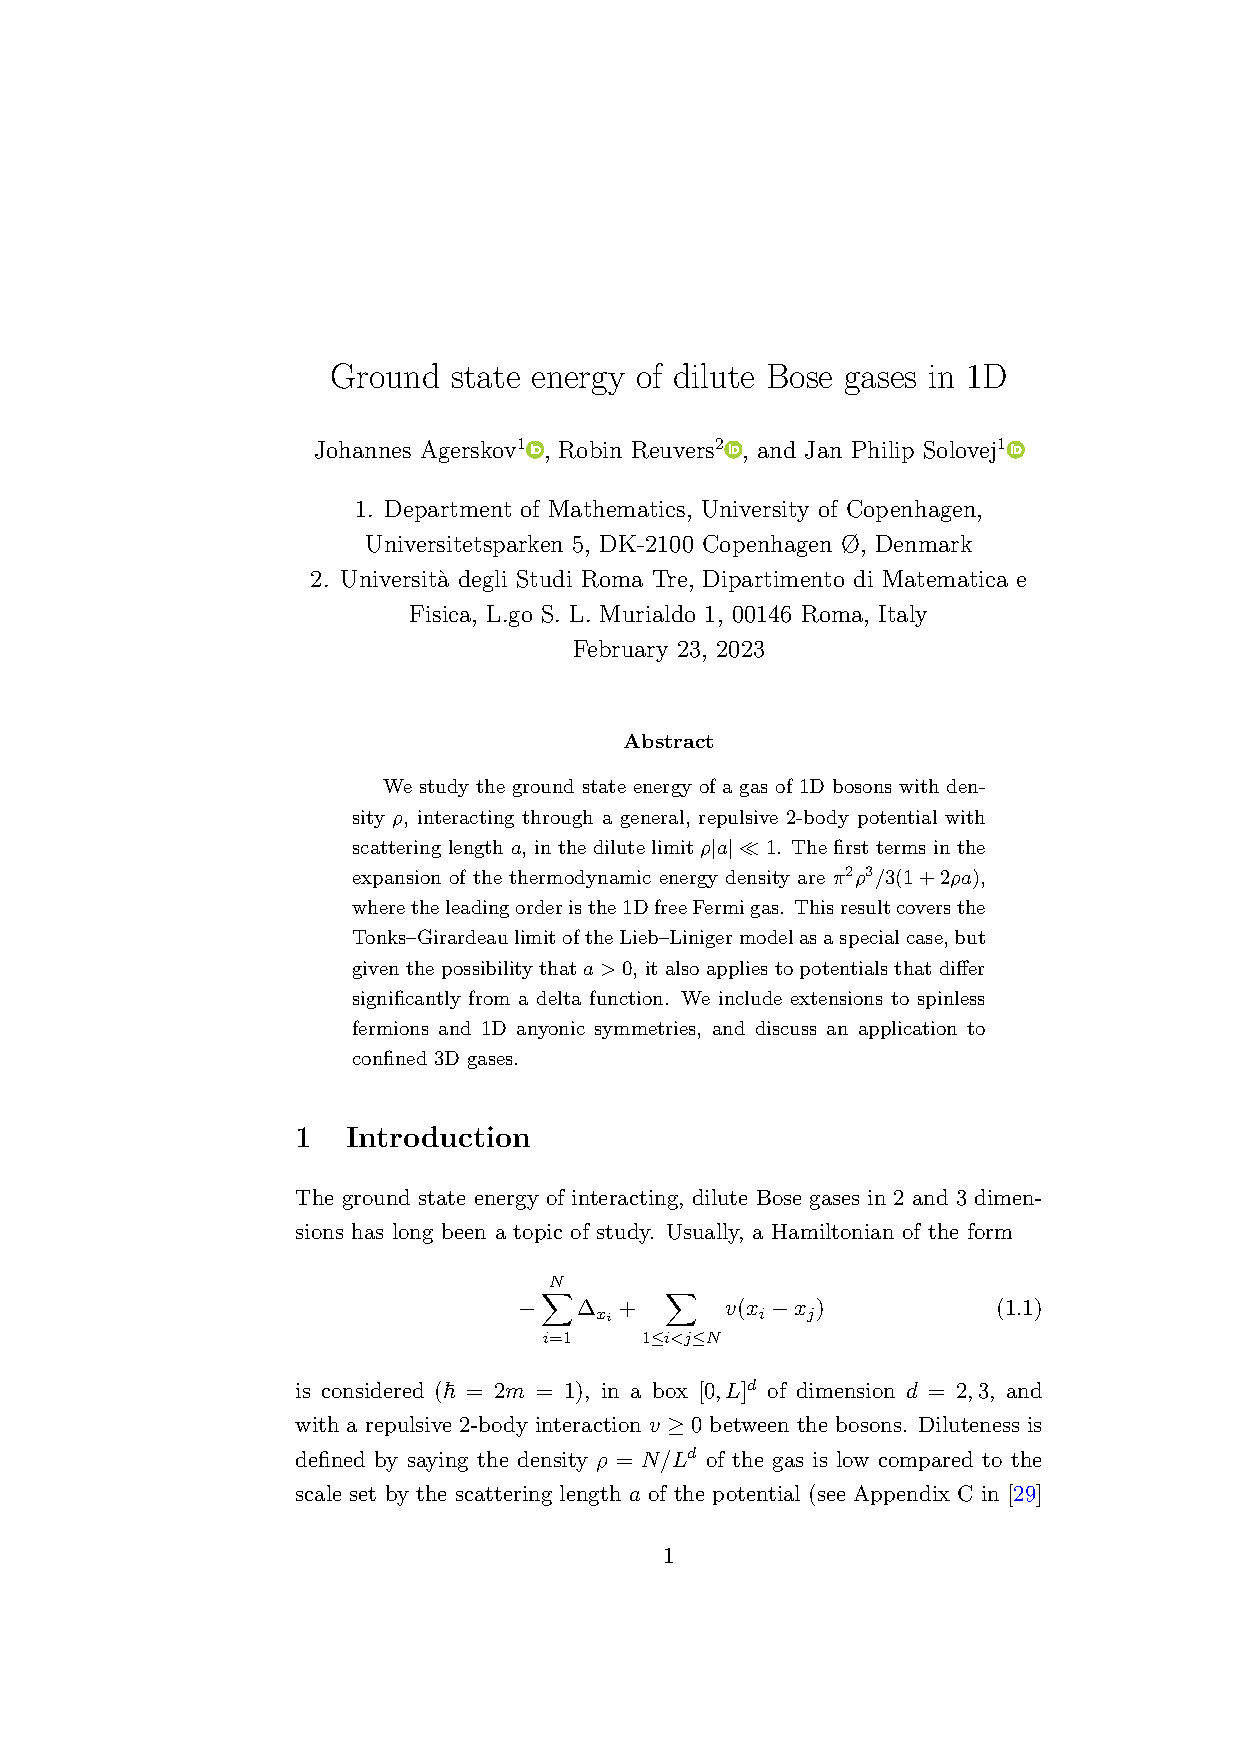
\includepdf[pages={1-},pagecommand={}]{/home/johannes/Documents/Phd/1d bosons draft/one_d_bosons_vThesis.pdf}


\bibliographystyle{alpha}
\bibliography{bibliography}
\end{document}
